\documentclass[conference,a4paper]{IEEEtran}

\usepackage[utf8]{inputenc}
\usepackage{cite}
\usepackage{amsmath,amssymb,amsfonts}
\usepackage{graphicx}
\usepackage{textcomp}
\usepackage{xcolor}
\usepackage{booktabs}
\usepackage{array}
\usepackage{url}
\usepackage{multirow}
\usepackage{tikz}
\usepackage{placeins}
\renewcommand{\ttdefault}{cmtt}
\usetikzlibrary{arrows.meta,positioning}
\graphicspath{{figures/}}

\def\BibTeX{{\rm B\kern-.05em{\sc i\kern-.025em b}\kern-.08em
    T\kern-.1667em\lower.7ex\hbox{E}\kern-.125emX}}

\begin{document}

\title{Benchmark Before You Automate: Leakage-Aware Evaluation of Machine Learning Detectors for Power-Sector SCADA Security}

\author{
\IEEEauthorblockN{Digdarshan Subedi}
\IEEEauthorblockA{
Department of Computer Science\\
University of Wisconsin--Whitewater\\
Whitewater, WI, USA\\
\textit{SubediD30@uww.edu}
}
\and
\IEEEauthorblockN{Nikesh Tiwari}
\IEEEauthorblockA{
School of Business \& Technology\\
Webster University\\
St. Louis, MO, USA\\
\textit{nikeshtiwari@webster.edu}
}
\and
\IEEEauthorblockN{Bibek Ale}
\IEEEauthorblockA{
School of Business \& Technology\\
Webster University\\
St. Louis, MO, USA\\
\textit{Bibekale@webster.edu}
}
}

\maketitle

\begin{abstract}
Power-grid operators are increasingly using machine learning to identify cyberattacks and support faster security response. As these systems move closer to semi-automated or automated operation, evaluation errors can become operational risks: an overstated model may trigger unnecessary protective actions or fail to detect a real intrusion. We examine a common evaluation practice on the MSU/ORNL power-system attack dataset, which contains fifteen independently sampled runs from the same testbed. When these runs are merged and split randomly, highly similar records from the same run can appear in both training and test sets. We compare this conventional protocol with a leakage-controlled, run-level evaluation that holds out one complete run at a time. Three lightweight detectors---Random Forest, XGBoost, and a feature-space one-dimensional convolutional network---are evaluated under both protocols. Random Forest achieved the strongest random-split result with F1=0.945 and ROC-AUC=0.972, but its run-level mean fell to F1=0.807 and ROC-AUC=0.677, absolute decreases of 0.138 and 0.296. XGBoost showed a similar reduction, while the CNN's F1 was stable but paired with near-chance ROC-AUC and a very high false-positive rate. We also use permutation importance and SHAP to identify the relay and phasor signals that drive detection. The findings show why leakage-aware evaluation should be treated as a prerequisite for trusting SCADA detectors in automated security workflows.
\end{abstract}

\begin{IEEEkeywords}
SCADA security, intrusion detection, data leakage, grouped cross-validation, cyber-physical systems, explainable machine learning
\end{IEEEkeywords}

\section{Introduction}

Power-grid operators must interpret large streams of relay, breaker, control-panel, and phasor measurements while also responding to cyber incidents that can affect physical equipment. Machine learning can help by ranking alerts, detecting unusual behavior, and supporting faster intervention. However, as detection becomes more closely connected to automated response, the cost of an incorrect prediction also increases. A false alarm may lead to an unnecessary relay isolation or breaker action, while a missed attack may continue through an unattended workflow. In this setting, model evaluation is not only a benchmarking exercise; it is part of the safety case for deployment.

A widely used benchmark for this task is the Mississippi State University/Oak Ridge National Laboratory (MSU/ORNL) power-system attack dataset~\cite{beaver2013power,pan2015classification}. It combines time-synchronized phasor measurements with relay, control-panel, and intrusion-detection logs from a physical power-system testbed. The data are distributed across fifteen independently sampled runs of the same scenario set. In much of the prior work, the runs are merged before a random row-level train/test split is created.

This evaluation practice introduces a mismatch between the benchmark and the intended deployment setting. Records from the same run share the same operating conditions, injected events, and closely related measurements. A random split can therefore place highly similar records in both training and test data. The resulting score may reflect recognition of familiar run-specific patterns rather than reliable detection under unseen conditions.

We study this mismatch directly. Rather than proposing a more complex detector, we ask how much reported performance changes when complete runs are held out during testing. We compare the conventional random split with a leakage-controlled protocol based on run-level cross-validation. The comparison is designed to answer a practical question: does a detector continue to perform well when it is evaluated on a run that was never represented during training?

We investigate three research questions:

\begin{itemize}
\item \textbf{RQ1.} How well do three lightweight detectors---Random Forest, XGBoost, and a feature-space 1D-CNN---identify attacks under the conventional random-split protocol?
\item \textbf{RQ2.} How much performance is retained when entire collection runs are held out, and is the change consistent across model families?
\item \textbf{RQ3.} Which physically meaningful relay and phasor measurements drive the predictions, and how might these explanations support operator review?
\end{itemize}

This paper makes four contributions:
\begin{itemize}
\item We formalize a run-level evaluation protocol that prevents records from the same collection run from appearing in both training and test data.
\item We measure the naive-versus-controlled performance gap across bagging, boosting, and convolutional models.
\item We interpret this gap as evidence about whether reported detector performance is strong enough to support automated security decisions.
\item We connect predictions to physically meaningful SCADA and PMU signals through permutation importance and SHAP.
\end{itemize}

\section{Related Work}

\subsection{Evaluating the MSU/ORNL Benchmark}

The MSU/ORNL dataset was introduced to support reproducible research on malicious SCADA communication and power-system disturbances~\cite{beaver2013power,pan2015classification}. Its value comes from combining cyber events with measurements from a physical relay, breaker, generator, and transmission-line testbed. However, the benchmark is organized as multiple independently sampled runs of the same scenario family. When those runs are pooled before random splitting, the evaluation may reward similarity to previously seen operating conditions.

Grouped evaluation is commonly used in machine learning when observations from the same subject, session, device, or experimental run are correlated. Its purpose is simple: all records from one group are kept on the same side of the train/test boundary. In this work, we apply that principle at the collection-run level so that the test set more closely represents unseen operating data.

\subsection{Machine Learning for Power-System Intrusion Detection}

Prior work on grid and SCADA intrusion detection includes decision trees, ensemble models, neural networks, and hybrid systems. Tree-based methods remain attractive because they are inexpensive to train, work well on tabular telemetry, and provide useful feature rankings. Deep models can capture more complex relationships, but they may also require more data, more tuning, and stronger assumptions about sequence or topology.

Smart-grid security and data-analytics surveys identify recurring challenges for data-driven grid protection, including limited labeled data, changing operating conditions, and the need for validation that matches deployment conditions~\cite{tan2017survey,wang2019deep}. Explanation methods such as SHAP can make model behavior easier to inspect~\cite{lundberg2017shap}. Our work addresses a more basic requirement: before an explanation can support operator trust, the underlying performance estimate must itself be credible.

\subsection{From Detection Accuracy to Automation Readiness}

AI-assisted grid monitoring raises the importance of evaluation design. A model used only as an analyst aid may tolerate some uncertainty because a human can review its output. A model connected to automated actions requires stronger evidence that its performance transfers beyond familiar data.

In contrast to work that mainly introduces new model architectures, we focus on the evaluation boundary itself. We ask whether reported performance survives when the test set is separated from the training set at the run level, and we treat the answer as evidence about automation readiness rather than only predictive accuracy.

\section{Methodology}

\subsection{Dataset and Classification Task}

We use the binary MSU/ORNL Power System Attack Dataset~\cite{beaver2013power,pan2015classification}. It contains fifteen independently sampled runs, stored as \texttt{data1.csv} through \texttt{data15.csv}, from one physical testbed. The testbed includes two generators, four relays, four breakers, and two transmission lines. All fifteen files were loaded separately before merging, and each record was tagged with its source run.

The dataset contains thirty-seven event scenarios: eight natural events, one normal-operation scenario, and twenty-eight attack scenarios. The public binary CSV files used here store the marker field as \texttt{Attack} or \texttt{Natural}, rather than preserving the original numeric scenario/load marker. We therefore verified the available binary labels and used the official README for the scenario mapping shown in Table~\ref{tab:labels}. The marker column is used only to derive the target and is excluded from model inputs.

\begin{table}[htbp]
\caption{Binary label mapping from the official dataset documentation. The public binary CSV files used in this study expose the label as Attack/Natural rather than preserving the numeric scenario marker.}
\label{tab:labels}
\centering
\scriptsize
\begin{tabular*}{\columnwidth}{@{\extracolsep{\fill}}p{0.22\columnwidth}p{0.70\columnwidth}}
\toprule
\textbf{Label} & \textbf{Scenario Numbers} \\
\midrule
Attack (1) & 7--12, 15--30, 35--40 \\
Non-attack (0) & 1--6, 13, 14, 41 \\
\bottomrule
\end{tabular*}
\end{table}

The fifteen files represent repeated samples from the same testbed, not separate physical sites. We therefore make claims about run-level generalization only. We do not claim cross-site, cross-vendor, or cross-topology generalization. The combined corpus contains 78,377 records: 55,663 attacks and 22,714 non-attacks.

\subsection{Input Features}

Each record contains 128 input features after excluding the marker field and added provenance columns. Of these, 116 are PMU measurements: twenty-nine signal types from each of four relay/PMU units. The remaining twelve features come from the control panel, Snort, and relay logs. We preserve the original physical labels so that feature-importance results remain interpretable to power-system readers.

\begin{table}[htbp]
\caption{Physical meaning of the PMU feature groups. Each signal appears for relays R1--R4.}
\label{tab:features}
\centering
\scriptsize
\setlength{\tabcolsep}{4pt}
\begin{tabular*}{\columnwidth}{@{\extracolsep{\fill}}p{0.30\columnwidth}p{0.62\columnwidth}}
\toprule
\textbf{Signal} & \textbf{Description} \\
\midrule
PA1:VH--PA3:VH & Phase A--C voltage phase angle \\
PM1:V--PM3:V & Phase A--C voltage magnitude \\
PA4:IH--PA6:IH & Phase A--C current phase angle \\
PM4:I--PM6:I & Phase A--C current magnitude \\
PA7:VH--PA9:VH & Sequence voltage angle \\
PM7:V--PM9:V & Sequence voltage magnitude \\
PA10:VH--PA12:VH & Sequence current angle \\
PM10:V--PM12:V & Sequence current magnitude \\
F & Frequency \\
DF & Frequency change \\
PA:Z & Apparent impedance \\
PA:ZH & Apparent impedance angle \\
S & Relay status flag \\
\bottomrule
\end{tabular*}
\end{table}

\subsection{Detectors}

We select three models that are computationally practical for operational-technology environments and structurally different enough to test whether the evaluation effect is model-specific.

\textit{Random Forest} uses 200 trees and provides a strong tabular baseline. Its bagging structure reduces variance and offers direct feature-importance estimates.

\textit{XGBoost}~\cite{chen2016xgboost} also uses 200 estimators but learns through sequential boosting. Comparing it with Random Forest helps distinguish a dataset-level evaluation effect from behavior specific to one ensemble method.

\textit{Feature-space 1D-CNN} applies convolution across the ordered feature vector. Features are arranged by relay group---R1, R2, R3, R4---followed by control-panel and log features. The convolution is therefore intended to capture local relationships among physically co-located measurements.

The CNN is not a temporal model. The dataset was randomly sampled from the original recording, so row order does not represent a continuous time sequence. For this reason, we do not use LSTM or sequence-window models. Doing so would risk learning arbitrary sample order rather than grid dynamics.

\subsection{Evaluation Protocols}

The paper compares two protocols that use the same dataset, features, and models but differ in how test data are isolated.

\textit{Conventional random split.} All fifteen runs are merged, after which a stratified random 70/30 row-level train/test split is created with seed 42. This setting matches the common benchmark practice and serves as the baseline.

\textit{Leakage-controlled run-level split.} We apply fifteen-fold \texttt{GroupKFold} cross-validation using the source run as the grouping variable. Each fold trains on fourteen runs and tests on the remaining run. No record from the held-out run appears in training.

For both protocols, we report precision, recall, F1, false-positive rate, ROC-AUC, and confusion matrices. For the run-level protocol, we also report the mean and standard deviation across folds so that run-to-run variability remains visible. Median imputation is fitted only on training data. The CNN also uses training-only standardization and an internal validation split from the training runs for early stopping.

\subsection{Interpreting Model Decisions}

We use permutation importance for the best controlled-discrimination tree model and SHAP values for Random Forest and XGBoost using \texttt{TreeExplainer}~\cite{lundberg2017shap}. SHAP is not applied to the CNN because \texttt{TreeExplainer} is specific to tree models. We report this boundary explicitly and use physical feature names rather than anonymous feature indices.

\section{Results}

\subsection{Conventional Evaluation Suggests Strong Detection}

Table~\ref{tab:naive} reports the conventional random-split results. Random Forest led the random-split evaluation with F1=0.945 and ROC-AUC=0.972. Its F1 was 0.036 higher than XGBoost and 0.114 higher than the feature-space CNN. This result is strong under the conventional benchmark boundary, but the split allows records from each run to appear on both sides of the train/test divide.

\begin{table}[htbp]
\caption{Detection performance under the conventional random split. These values show how the models perform when records from the same run may appear in both training and test data.}
\label{tab:naive}
\centering
\scriptsize
\begin{tabular}{lccccc}
\toprule
\textbf{Model} & \textbf{Prec.} & \textbf{Rec.} & \textbf{F1} & \textbf{FPR} & \textbf{ROC-AUC} \\
\midrule
Random Forest & 0.915 & 0.976 & 0.945 & 0.224 & 0.972 \\
XGBoost & 0.871 & 0.950 & 0.908 & 0.346 & 0.922 \\
Feature-space CNN & 0.710 & 1.000 & 0.831 & 1.000 & 0.558 \\
\bottomrule
\end{tabular}
\end{table}
\FloatBarrier

\subsection{Run-Level Holdout Tests Transfer to Unseen Collections}

Table~\ref{tab:groupkfold} reports the mean and standard deviation across the fifteen held-out runs. The CNN had the highest mean F1 at 0.829$\pm$0.029, but its ROC-AUC was only 0.527$\pm$0.038 and its mean false-positive rate was 0.998. This means the CNN's F1 is largely explained by predicting the majority attack class rather than by strong discrimination. XGBoost had the strongest run-level ROC-AUC at 0.704$\pm$0.028, while Random Forest had a similar F1 but lower ROC-AUC.

\begin{table}[htbp]
\caption{Detection performance under leakage-controlled evaluation, reported as mean $\pm$ standard deviation across fifteen held-out runs.}
\label{tab:groupkfold}
\centering
\scriptsize
\resizebox{\columnwidth}{!}{%
\begin{tabular}{lccccc}
\toprule
\textbf{Model} & \textbf{Prec.} & \textbf{Rec.} & \textbf{F1} & \textbf{FPR} & \textbf{ROC-AUC} \\
\midrule
Random Forest & 0.760$\pm$0.035 & 0.861$\pm$0.012 & 0.807$\pm$0.018 & 0.667$\pm$0.028 & 0.677$\pm$0.029 \\
XGBoost & 0.763$\pm$0.038 & 0.853$\pm$0.009 & 0.805$\pm$0.022 & 0.650$\pm$0.038 & 0.704$\pm$0.028 \\
Feature-space CNN & 0.711$\pm$0.043 & 0.998$\pm$0.006 & 0.829$\pm$0.029 & 0.998$\pm$0.004 & 0.527$\pm$0.038 \\
\bottomrule
\end{tabular}
}
\end{table}
\FloatBarrier

\begin{figure}[!ht]
\centering
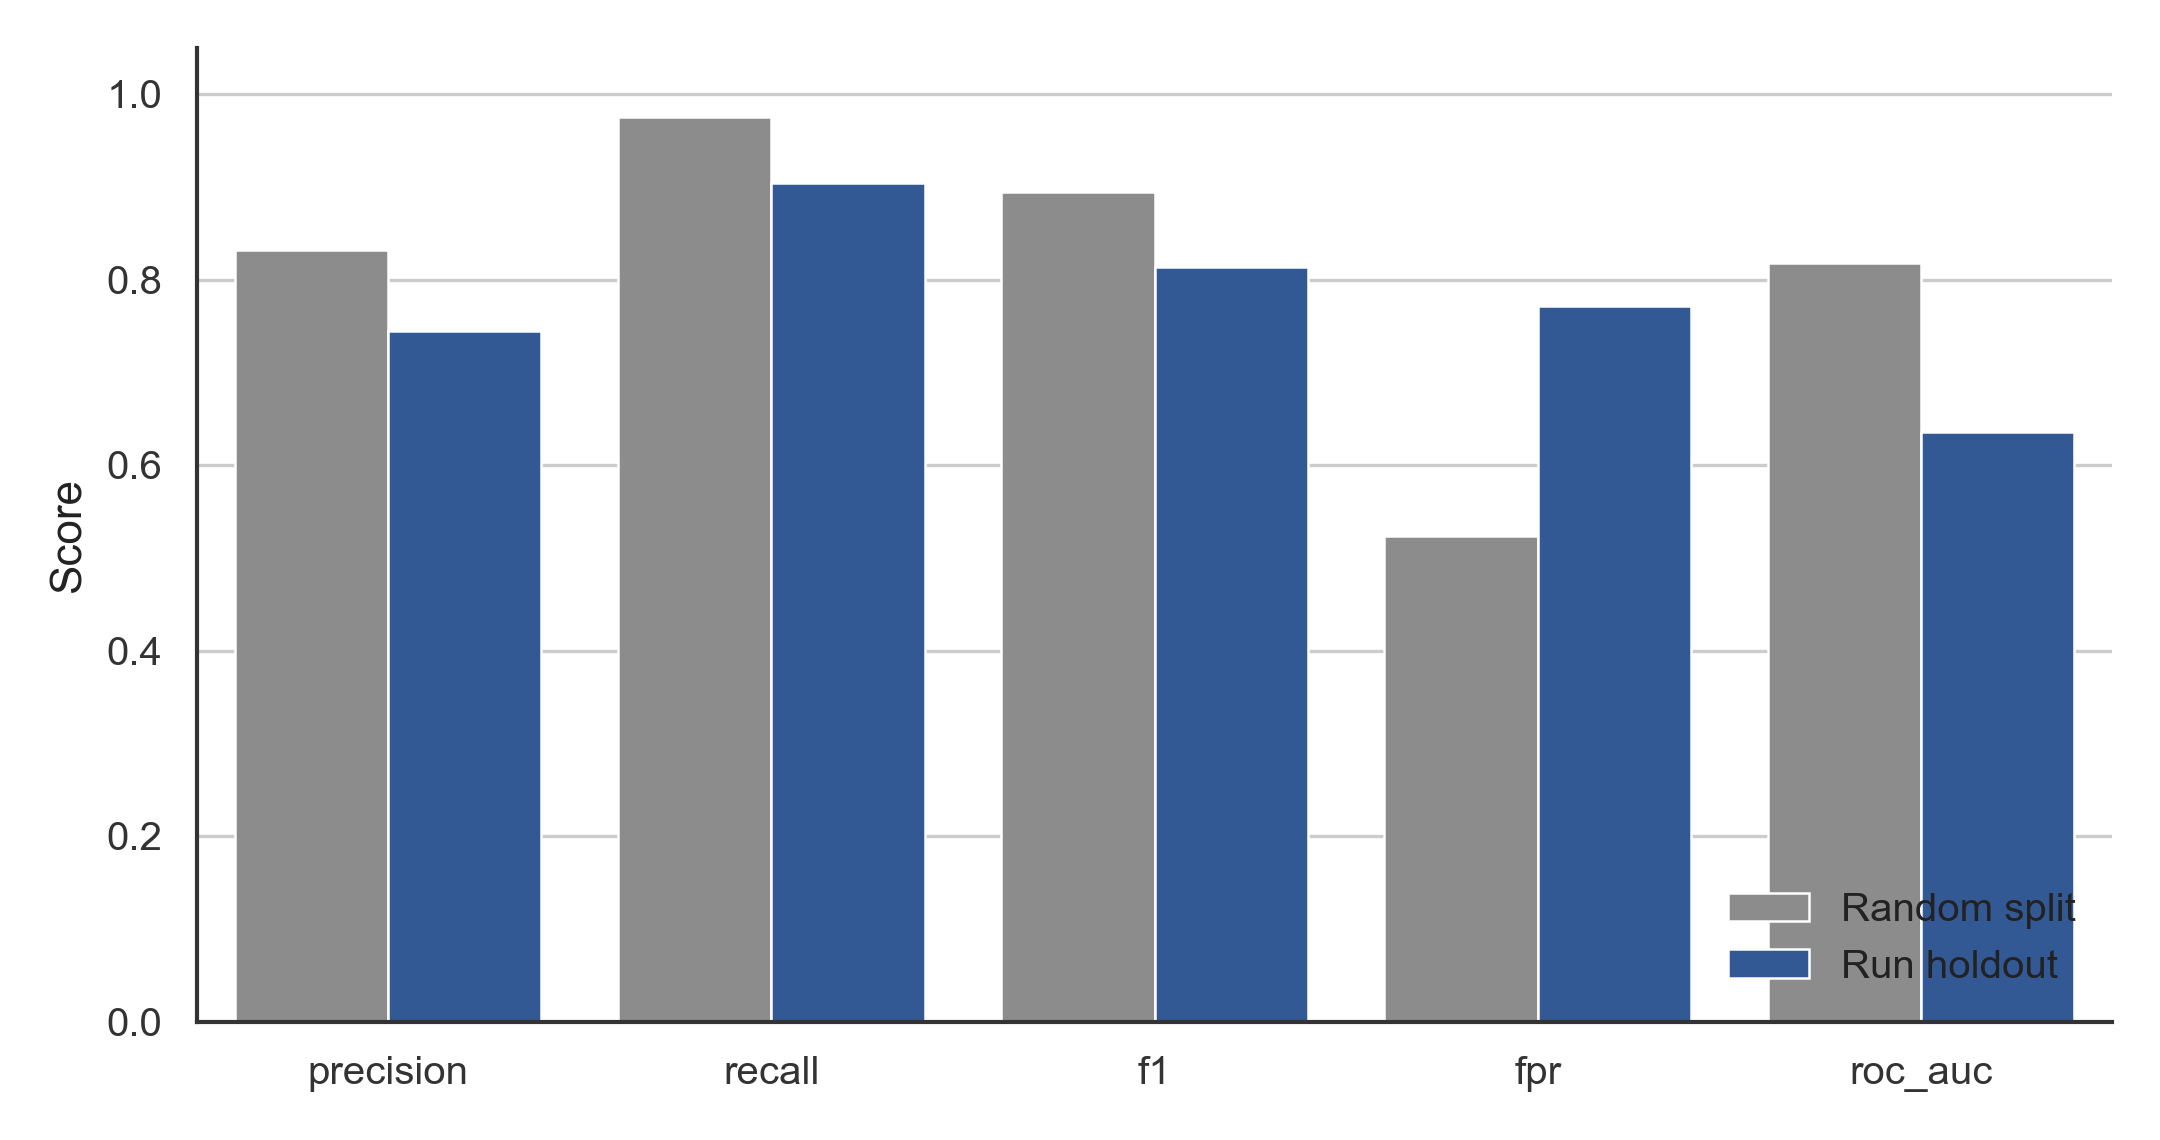
\includegraphics[width=\columnwidth]{fig1_naive_vs_leakage_metrics.png}
\caption{Comparison of the conventional random split and the leakage-controlled run-level protocol for all three detectors. The paired bars show whether performance measured on mixed-run test data is retained when the model is evaluated on a complete unseen run. The difference between the two bars is the paper's central measurement because it separates apparent benchmark performance from run-level transfer.}
\label{fig:naive_vs_leakage}
\end{figure}
\FloatBarrier

\begin{figure}[!ht]
\centering
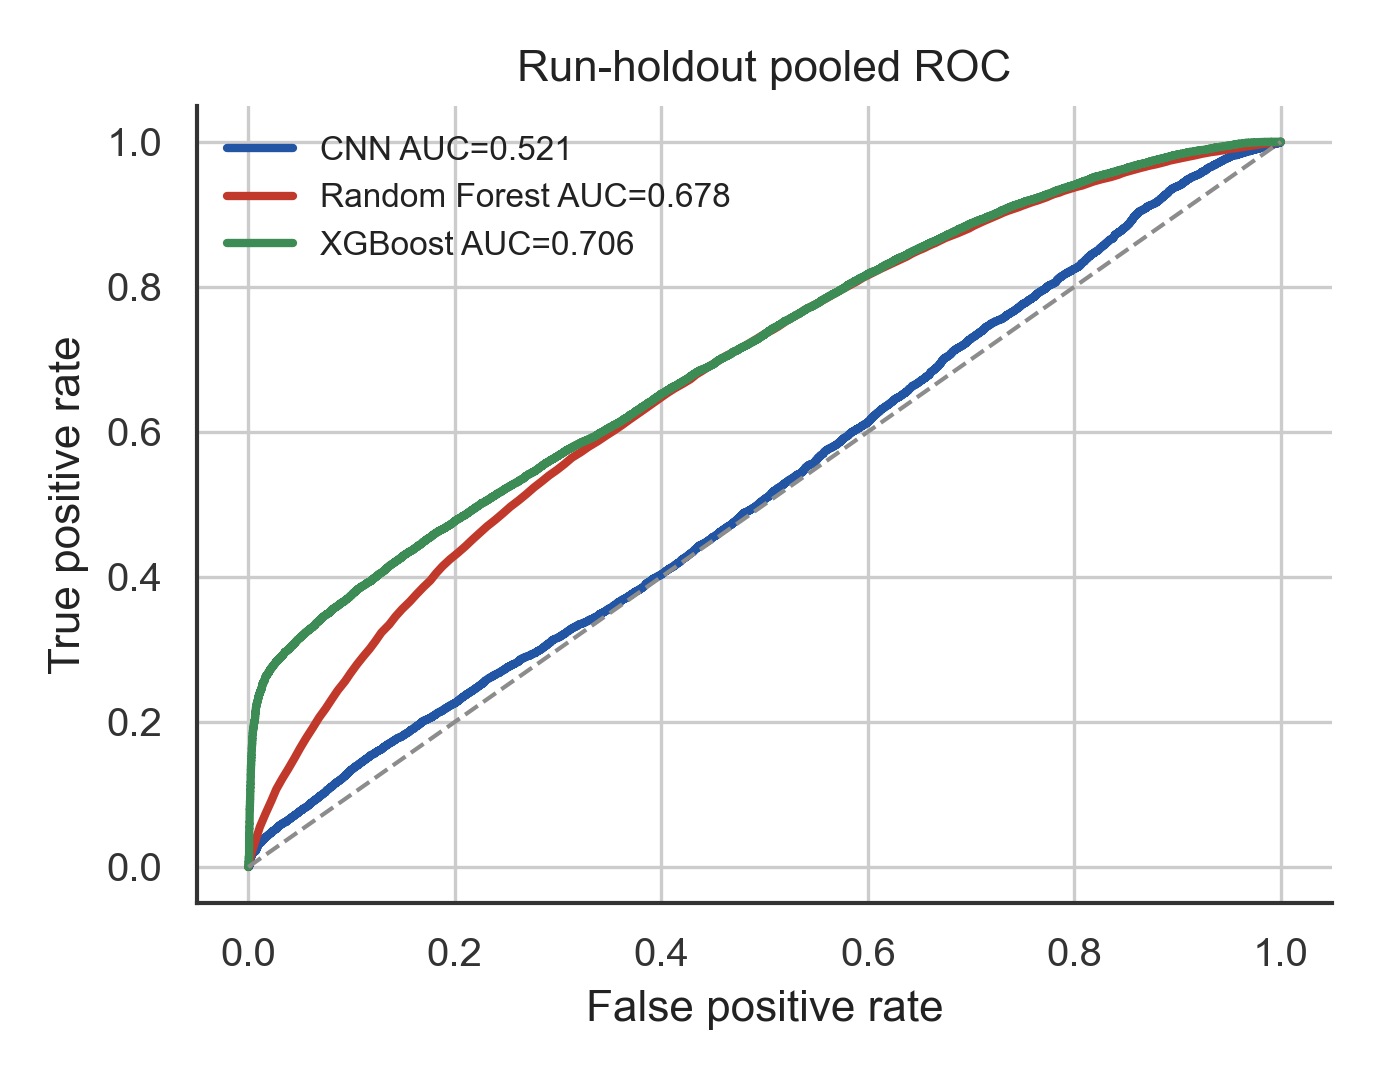
\includegraphics[width=\columnwidth]{fig3_roc_leakage.png}
\caption{Pooled ROC curves under run-level holdout. Each curve concatenates out-of-fold predictions from runs that were absent during training. XGBoost has the strongest controlled discrimination, while the CNN's curve shows why its high F1 must be interpreted cautiously.}
\label{fig:roc_leakage}
\end{figure}
\FloatBarrier

\subsection{The Evaluation Gap Quantifies Benchmark Optimism}

Table~\ref{tab:delta} isolates the F1 difference between protocols. Random Forest dropped by 0.138 F1 and 0.296 ROC-AUC under run-level holdout. XGBoost dropped by 0.103 F1 and 0.218 ROC-AUC. The CNN showed almost no F1 gap, but this does not indicate robust transfer because its ROC-AUC was low under both protocols and its false-positive rate was nearly one. For the two discriminative tree models, the pattern is consistent: conventional random splitting reports substantially higher performance than run-level holdout.

\begin{table}[htbp]
\caption{F1 under each protocol and the resulting evaluation gap. A positive gap indicates that the conventional random split reports higher performance than the run-level protocol.}
\label{tab:delta}
\centering
\scriptsize
\begin{tabular*}{\columnwidth}{@{\extracolsep{\fill}}lccc}
\toprule
\textbf{Model} & \textbf{Naive F1} & \textbf{Run-Level F1} & \textbf{$\Delta$F1} \\
\midrule
Random Forest & 0.945 & 0.807 & 0.138 \\
XGBoost & 0.908 & 0.805 & 0.103 \\
Feature-space CNN & 0.831 & 0.829 & 0.001 \\
\bottomrule
\end{tabular*}
\end{table}

\begin{figure}[!ht]
\centering
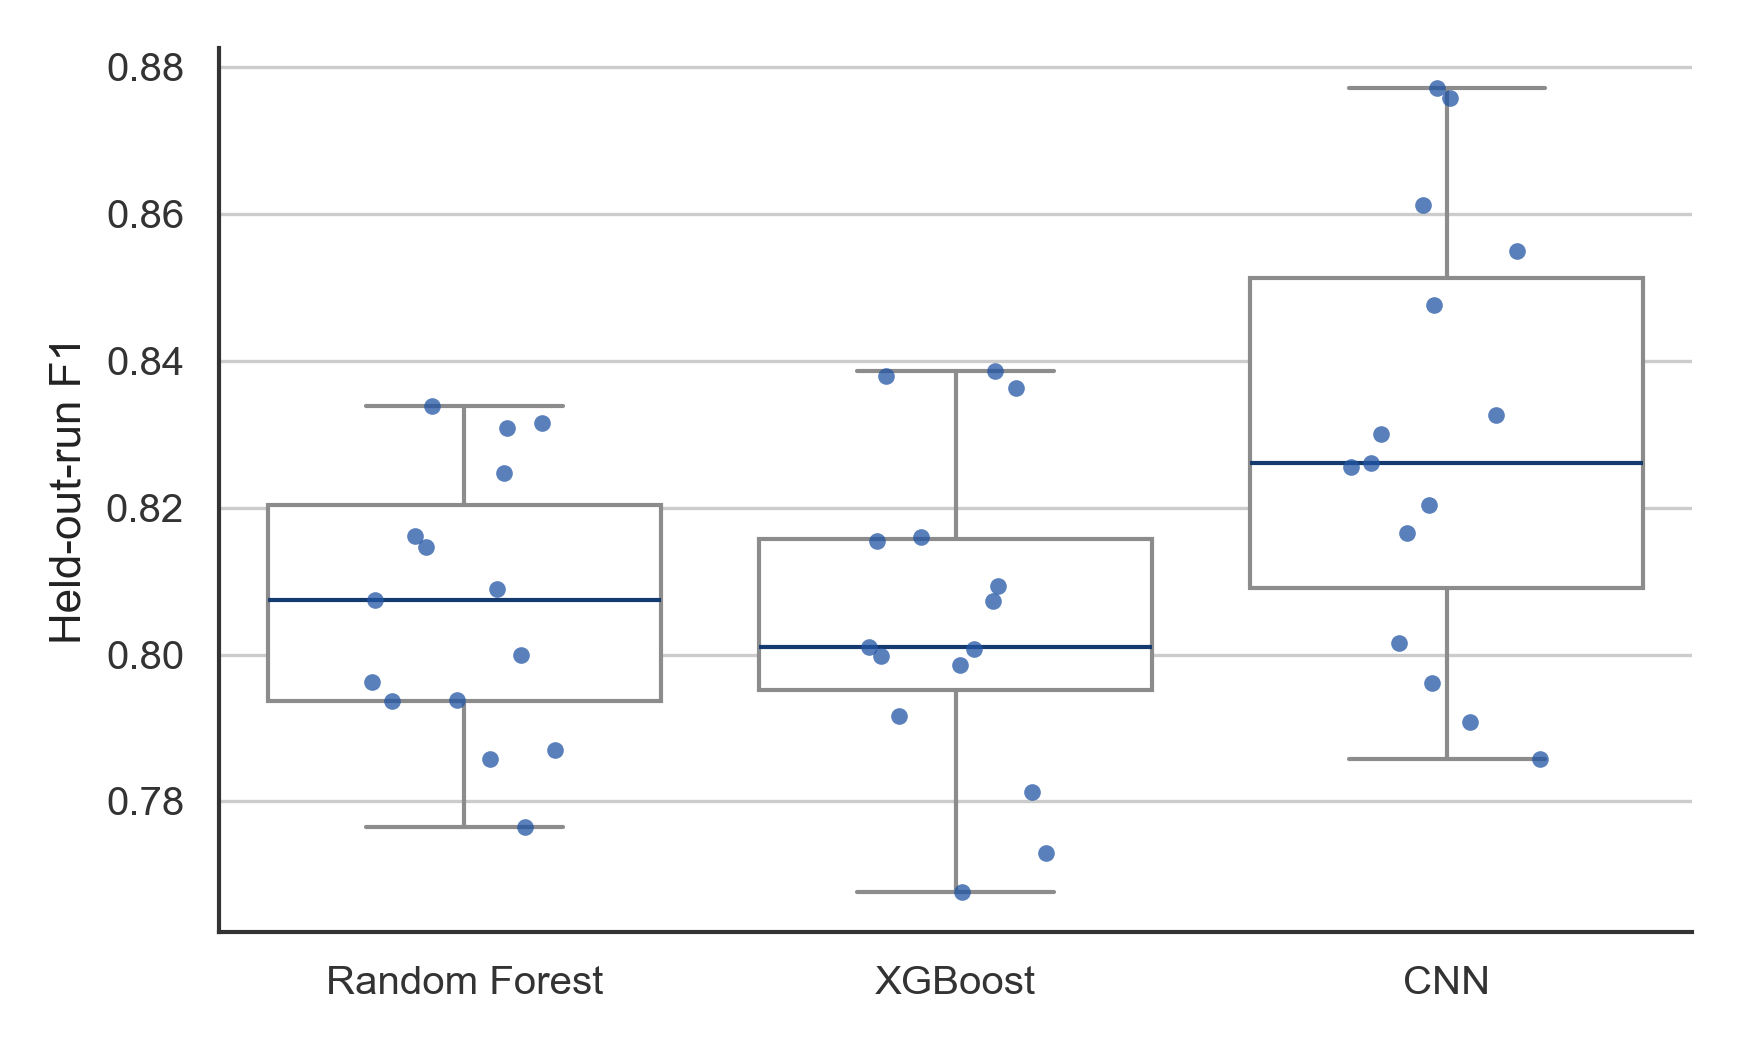
\includegraphics[width=\columnwidth]{fig5_fold_variance.png}
\caption{Per-fold F1 across the fifteen held-out runs. Each value corresponds to a model tested on one complete run that was absent from training. Wide dispersion indicates that detection difficulty varies across collections and that a single random split may conceal this variation.}
\label{fig:fold_variance}
\end{figure}
\FloatBarrier

\begin{figure}[!ht]
\centering
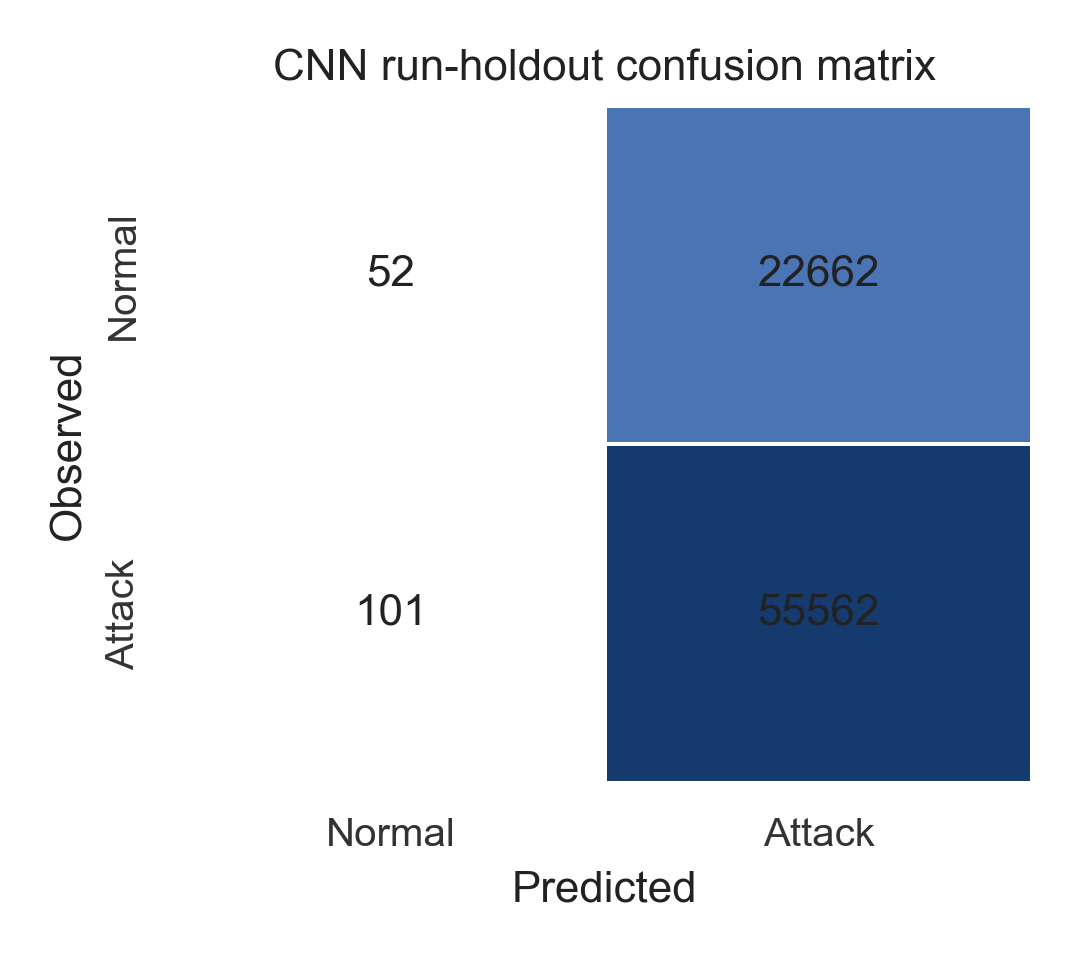
\includegraphics[width=.86\columnwidth]{fig4_confusion_matrix.png}
\caption{Pooled run-level confusion matrix for the best controlled-F1 model. The large number of false positives explains why F1 alone overstates the CNN's usefulness for operational review.}
\label{fig:confusion}
\end{figure}
\FloatBarrier

\subsection{Physically Meaningful Signals Support Operator Review}

Fig.~\ref{fig:importance} reports the leading held-out feature-importance values. The strongest permutation features include R4-PM2:V, R2-PM1:V, R2-PM4:I, R4-PA:ZH, R3-PA:Z, and R1-PA:ZH. These features are voltage magnitude, current magnitude, and impedance-related relay/PMU measurements, which are plausible for distinguishing physical disturbances and command/data attacks. SHAP was computed only for tree models; it broadly emphasized relay and phasor quantities rather than artificial identifiers. This agreement supports the interpretability of the detector behavior, but it does not prove causal detection.

\begin{figure}[!ht]
\centering
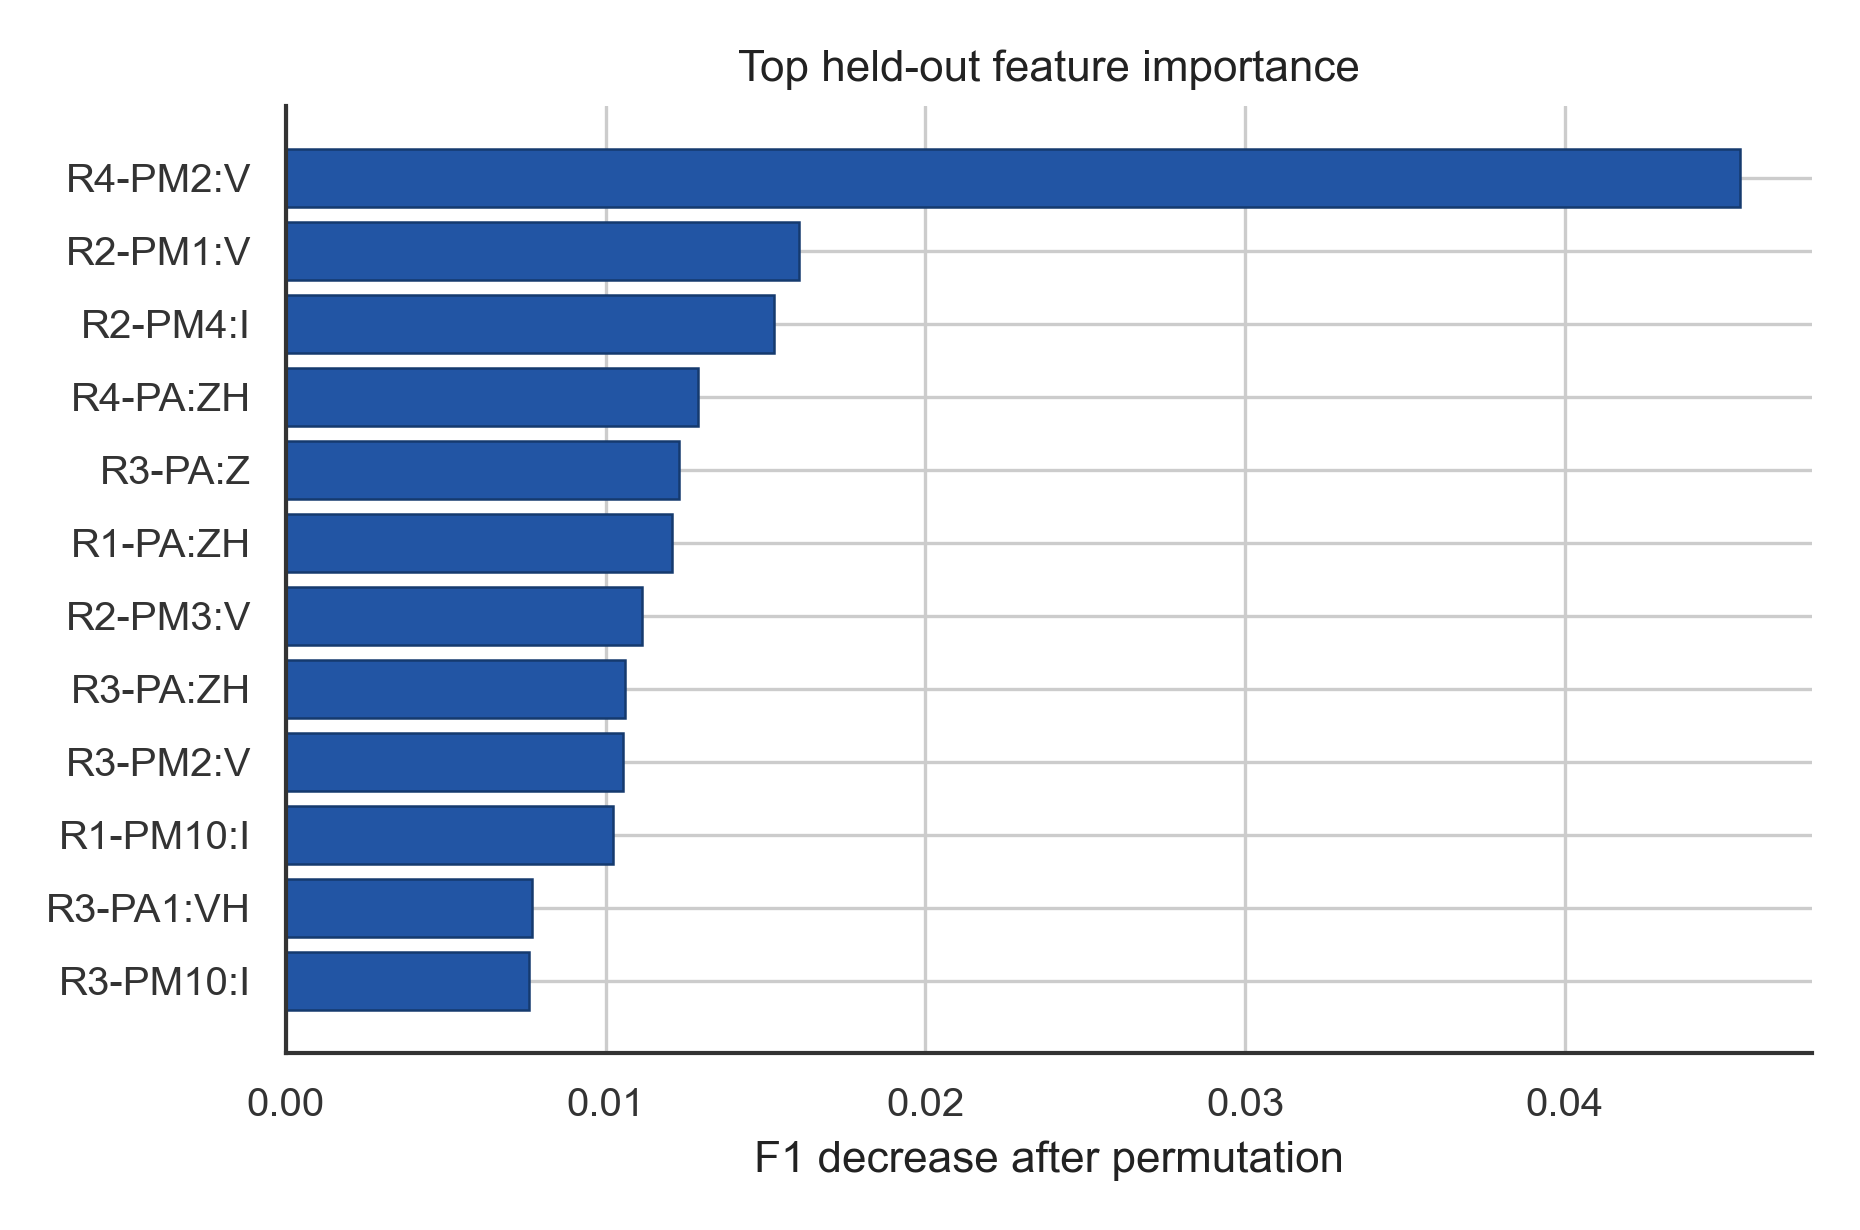
\includegraphics[width=\columnwidth]{fig6_feature_importance.png}
\caption{Top features identified through held-out permutation importance and tree-model SHAP analysis. Features are labeled using their physical PMU or relay meaning rather than anonymous column indices. Agreement around voltage, current, and impedance quantities suggests that the tree models rely on interpretable grid measurements, although attribution does not establish causality.}
\label{fig:importance}
\end{figure}
\FloatBarrier

\section{Discussion}

\subsection{Automation Readiness Depends on the Score That Survives Holdout}

The practical question is not which model achieves the largest number under the easiest split. It is whether the reported score remains credible when the model faces data from an unseen run. Random Forest reached F1=0.945 and ROC-AUC=0.972 under the random split, but only F1=0.807 and ROC-AUC=0.677 under run-level holdout. XGBoost showed the same direction of change, from F1=0.908 and ROC-AUC=0.922 to F1=0.805 and ROC-AUC=0.704.

This distinction matters because automated security workflows act on predictions rather than benchmark tables. A large gap means that a detector certified using the conventional split may appear more reliable than it is under deployment-like conditions. A small gap would support a different conclusion: the benchmark is more robust to run-level overlap than its structure suggests. In either case, the run-level result is the more defensible basis for deployment decisions.

\subsection{The Gap Is Not Explained by a Large Loss of Training Data}

A reasonable concern is that run-level cross-validation may lower performance simply because each fold uses less training data. The opposite is true here: the random split trained on 54,863 records, while each grouped fold trained on an average of 73,152 records, or 93.3\% of the available corpus. The more important change is the relationship between training and test records. Under the random split, similar records from the same run may appear on both sides. Under the grouped split, this overlap is structurally impossible.

For this reason, a systematic performance reduction is better interpreted as evidence of run-level dependence than as a simple sample-size effect. The fold-level variance provides a second signal: if some runs are consistently harder than others, a single random split can mask that heterogeneity.

\subsection{Interpretability Helps Review, but Does Not Replace Validation}

Feature attribution can help an operator understand why a detector raised an alert. For example, a decision driven by relay status, impedance, or abnormal phasor measurements is easier to inspect than one driven by opaque identifiers or dataset artifacts. However, a plausible explanation does not prove that a model generalizes. Interpretability and leakage control address different questions: one concerns why a prediction was made, while the other concerns whether the reported performance can be trusted.

\subsection{The Contribution Is an Evaluation Standard, Not a New Architecture}

The value of this work lies in separating model quality from evaluation convenience. The same run-level protocol can be applied to future tree, graph, attention, or hybrid detectors. This makes the contribution transferable even though the present study evaluates only three lightweight models.

\section{Limitations and Future Work}
\label{sec:limitations}

\textit{Dataset scope.} The study uses one 2014-era physical testbed. The results therefore describe run-level generalization within this benchmark, not transfer across utilities, vendors, grid topologies, or contemporary attack campaigns. Future work should repeat the protocol on multi-site and multi-testbed datasets.

\textit{Method scope.} We evaluate three deployable model families rather than conducting an exhaustive architecture search. Graph neural networks and attention-based models could be tested under the same protocol. Temporal models require a different data product because the current dataset is randomly sampled and does not preserve contiguous sequence structure.

\textit{Explanation scope.} The present explanations are post-hoc feature attributions. Future work should evaluate whether operators can use these explanations during realistic incident triage, and whether locally hosted explanation interfaces can improve review without exposing sensitive OT telemetry.

\textit{Deployment scope.} This study does not connect predictions to live protective actions. A deployment study would need prospective testing, latency measurements, calibrated confidence thresholds, fail-safe controls, and explicit human-override procedures.

\section{Conclusion}

Machine-learning evaluation becomes a safety concern when detection is connected to automated response. This paper compares the conventional random split on the MSU/ORNL power-system attack dataset with a leakage-controlled protocol that holds out complete collection runs. Across Random Forest, XGBoost, and a feature-space 1D-CNN, the comparison measures how much reported performance survives under a more deployment-relevant boundary. The best random-split result was Random Forest with F1=0.945 and ROC-AUC=0.972. Under run-level holdout, the highest F1 was 0.829 for the CNN, but the strongest controlled ROC-AUC was XGBoost at 0.704; the Random Forest and XGBoost F1 gaps were 0.138 and 0.103, respectively. The results support a simple recommendation: SCADA intrusion-detection studies should report grouped, run-level evaluation alongside conventional splits before presenting a model as suitable for autonomous or semi-autonomous operation.

\bibliographystyle{IEEEtran}
\bibliography{references}

\end{document}
